\section{The Unified Field Equation (UFE)}
%=============================================================================

%-----------------------------------------------------------------------------
\subsection{Quantum Vacuum Tensor Packaging}
%-----------------------------------------------------------------------------

\begin{definition}{Quantum Vacuum Tensor}{QVT}
Let
\begin{equation}
Q_{AB} := \hat{R}_{AB}(\hat{\Gamma}),
\qquad
Q^{\mathrm{TF}}_{AB} := Q_{AB} - \frac{1}{D}\hat{g}_{AB} Q^{C}{}_{C},
\qquad D:=4+n.
\end{equation}
Let $I(\alpha,L)$ denote the scalar invariant entering the coupling equation,
\begin{equation}
I(\alpha,L) := \alpha^3 - 2\cthree^3\alpha^2 - 8 \bone \cthree^6 L,
\qquad L := \ln\!\left(\frac{1}{\phiz(\alpha)}\right).
\end{equation}
Define the Quantum Vacuum Tensor
\begin{equation}
V_{AB} := Q^{\mathrm{TF}}_{AB} + \hat{g}_{AB}\, I(\alpha,L).
\end{equation}

\tcblower
\textbf{Structural equivalence principle (packaging statement).}
The vacuum law $V_{AB}=0$ splits into a scalar channel $I(\alpha,L)=0$ (CFE closure)
and a traceless ($D$-dimensional) channel $Q^{\mathrm{TF}}_{AB}=0$ (torsion vacuum equation).
This provides a compact bridge between the scalar and tensor sectors without introducing new inputs.
\end{definition}

%-----------------------------------------------------------------------------
\subsection{Torsionful Geometric Action}
%-----------------------------------------------------------------------------

\begin{definition}{UFE Action}{UFEaction}
On a manifold $M^{4+n}$ with metric $\hat{g}_{AB}$ and torsionful connection 
$\hat{\Gamma}^A_{BC}$, the action is:
\begin{equation}
    S = \int d^{4+n}x\sqrt{-\hat{g}}\left[
        \frac{1}{2\hat{\kappa}^2}\hat{R}(\hat{\Gamma}) 
        - \frac{1}{4}F_{AB}F^{AB}
        + \frac{1}{2}\hat{g}^{AB}\partial_A a\,\partial_B a 
        - V(a) 
        - \frac{\gagg}{4}\, a\, F_{AB}\tilde{F}^{AB}
    \right]
\end{equation}
Here $\hat{R}(\hat{\Gamma})$ denotes the Ricci scalar constructed from the full torsionful connection $\hat{\Gamma}$.
\end{definition}

\noindent\textbf{Minimal torsion sector.} In the parameter-free baseline we set $\mathcal{L}_{\mathrm{tors}}\equiv 0$.
All torsion dependence enters through $\hat{R}(\hat{\Gamma})$ with $\hat{\Gamma}=\Gamma(\hat{g})+K$.
The quadratic torsion treatment used for the one-loop $R^2$ completion is stated explicitly in Definition~\ref{def:R2torsion} and Appendix~\ref{app:r2}.

\noindent\textbf{Maxwell convention.} We treat the U(1) gauge potential $A$ as a one-form and define the field strength by the exterior derivative
$F := dA$, i.e.\ $F_{AB}=2\partial_{[A}A_{B]}$. This definition is independent of the torsionful affine connection $\hat{\Gamma}$; in particular, we do not use $F_{AB}=2\hat{\nabla}_{[A}A_{B]}$. Therefore U(1) gauge invariance is exact in the electromagnetic sector.

\noindent\textbf{Torsion and contorsion.} The torsion of the full connection is $T^A_{\;BC}:=2\hat{\Gamma}^A_{[BC]}$. We decompose
$\hat{\Gamma}^A_{BC}=\Gamma^A_{BC}(\hat{g})+K^A_{BC}$, where $\Gamma(\hat{g})$ is the Levi-Civita connection of $\hat{g}_{AB}$ and $K^A_{BC}$ is the contorsion tensor.

\noindent\textbf{Variational scope.} For the letter-level UFE statements we vary the metric while holding the torsionful connection fixed; no independent torsion equation of motion is required at this stage. In the core manuscript $K$ is treated as a background/auxiliary field (algebraic torsion can be integrated out); dynamical torsion is treated as an explicit extension.

\begin{theorem}{Unified Field Equations}{UFE}
Variation of the action yields the compact tensor form of the UFE. Since $\delta\hat{g}^{AB}$ is symmetric, only the symmetric part of the torsionful Ricci tensor contributes. Define
$\hat{G}_{(AB)}(\hat{\Gamma})$ by
\begin{equation*}
    \hat{G}_{(AB)}(\hat{\Gamma}) := \hat{R}_{(AB)}(\hat{\Gamma}) - \frac{1}{2}\hat{g}_{AB}\hat{R}(\hat{\Gamma}).
\end{equation*}
Then:
\begin{align}
    \hat{G}_{(AB)}(\hat{\Gamma})
        &= \hat{\kappa}^2\bigl(T^{(a)}_{AB} + T^{(\text{EM})}_{AB}\bigr)
        \label{eq:UFE}\\[0.5em]
    \nabla^{\mathrm{LC}}_A F^{AB} + \gagg(\partial_A a)\tilde{F}^{AB} &= 0
        \label{eq:maxwell}\\[0.5em]
    \nabla^{\mathrm{LC}}_A\tilde{F}^{AB} &= 0
        \label{eq:bianchi}
\end{align}
Here $\tilde{F}^{AB} := \tfrac12\,\epsilon^{ABCD}F_{CD}$ with $\epsilon^{0123}=+1$ and
metric signature $(+,-,-,-)$, and the coupling is $\gagg=-4\cthree$.
In Eqs.~\eqref{eq:maxwell}--\eqref{eq:bianchi} the covariant derivative is the Levi-Civita derivative of $\hat{g}_{AB}$ (equivalently $\nabla^{\mathrm{LC}}_A X^A=(1/\sqrt{-\hat{g}})\,\partial_A(\sqrt{-\hat{g}}\,X^A)$).
When expanding Eq.~\eqref{eq:UFE} in Levi-Civita plus contorsion variables (with $\hat{\Gamma}=\Gamma(\hat{g})+K$), all covariant derivatives are Levi-Civita.
In the torsion vacuum $(K \to 0)$, this reduces to Einstein--Hilbert gravity 
by Axiom A8.
\end{theorem}

\begin{tcolorbox}[colback=gray!5, colframe=gray!60,
title={\textbf{On-page variation for the axion--Maxwell term}}, fonttitle=\bfseries\small]
\textbf{Interaction:} $L_{\mathrm{int}}=-(\gagg/4)\,a\,F_{AB}\tilde{F}^{AB}$. \\
\textbf{Variation:} $\delta(F_{AB}\tilde{F}^{AB})=2\tilde{F}^{AB}\delta F_{AB}$ and $\delta F_{AB}=2\partial_{[A}\delta A_{B]}$. \\
\textbf{Result:} integrating by parts yields $\nabla_A F^{AB}+\gagg(\partial_A a)\tilde{F}^{AB}=0$,
matching Eq.~\eqref{eq:maxwell}.
\end{tcolorbox}

\begin{tcolorbox}[colback=gray!5, colframe=gray!60,
title={\textbf{Why the UFE uses the symmetric torsionful Einstein tensor}}, fonttitle=\bfseries\small]
Start from the torsionful Einstein--Hilbert term
\[
S_{\mathrm{EH}}=\frac{1}{2\hat{\kappa}^2}\int d^{4+n}x\,\sqrt{-\hat{g}}\;\hat{R},
\qquad
\hat{R}=\hat{g}^{AB}\hat{R}_{AB}(\hat{\Gamma}).
\]
Vary $\hat{g}^{AB}$ while holding $\hat{\Gamma}$ fixed:
\[
\delta\hat{R}=\hat{R}_{AB}\,\delta\hat{g}^{AB},
\qquad
\delta\sqrt{-\hat{g}}=-\frac12\sqrt{-\hat{g}}\;\hat{g}_{AB}\,\delta\hat{g}^{AB}.
\]
Hence $\delta S_{\mathrm{EH}}\propto\bigl(\hat{R}_{AB}-\tfrac12\hat{g}_{AB}\hat{R}\bigr)\delta\hat{g}^{AB}$.
Since $\delta\hat{g}^{AB}$ is symmetric, only the $(AB)$ part contributes, so the unambiguous vacuum equation is
\[
\hat{G}_{(AB)}(\hat{\Gamma})\equiv \hat{R}_{(AB)}(\hat{\Gamma})-\frac12\hat{g}_{AB}\hat{R}(\hat{\Gamma})=0.
\]
\end{tcolorbox}

\begin{tcolorbox}[colback=gray!5, colframe=gray!60,
title={\textbf{Notation: Ricci tensor under }\(\hat{\Gamma}=\Gamma(\hat{g})+K\)}, fonttitle=\bfseries\small]
We use $\nabla$ for the Levi-Civita derivative of $\hat{g}_{AB}$ in this decomposition.
Define the contracted rank-two tensors
\[
(\nabla K)_{BD}:=\nabla_A K^A{}_{DB}-\nabla_D K^A{}_{AB},
\qquad
(K^2)_{BD}:=K^A{}_{AE}K^E{}_{DB}-K^A{}_{DE}K^E{}_{AB}.
\]
With these conventions the identity is literal:
\[
\hat{R}_{BD}=R_{BD}+(\nabla K)_{BD}+(K^2)_{BD}.
\]
\end{tcolorbox}

\begin{tcolorbox}[colback=blue!3, colframe=blue!40,
    title={\textbf{Lemma (Torsion-Induced Bounce Term)}}, fonttitle=\bfseries\small]
In Einstein--Cartan-type setups where torsion is algebraic, integrating out the
axial torsion produces an effective spin--spin interaction
$(\bar{\psi}\gamma_5\gamma_\mu\psi)^2$. In a homogeneous cosmological background this term
scales as $a^{-6}$ and contributes a repulsive component at small scale factor,
allowing a non-singular bounce. This provides the minimal bridge from the UFE to
bounce scenarios used in Sec.~\ref{sec:bounce}.
\end{tcolorbox}

%-----------------------------------------------------------------------------
\subsection{Present-Day Torsion Regimes and Local Tests}
\label{sec:torsion-regimes}
%-----------------------------------------------------------------------------

TFPT distinguishes between \emph{cosmological torsion} (which may be active in the early universe and drive a bounce) and \emph{local vacuum torsion} (which is constrained by laboratory and astrophysical bounds on Lorentz violation).
To avoid hidden assumptions, we treat ``torsion today'' as an explicit regime choice rather than a vague qualitative statement.

\begin{tcolorbox}[colback=yellow!3, colframe=yellow!60!black,
    title={\textbf{Regime declaration (baseline vs.\ falsifiable alternatives)}}, fonttitle=\bfseries\small]
\textbf{Baseline (suite):} local vacuum torsion today vanishes,
\[
S_\mu(\text{today})=0,
\]
so local bounds are automatically satisfied and only cosmological torsion dynamics remain relevant for early-universe completions (bounce, condensates).

\textbf{Falsifiable alternatives:} if a TFPT completion predicts a nonzero local $S_\mu$, it must lie below the component-wise bounds and should be stated as a concrete regime proposal (the suite provides an exportable JSON ``regime designer'' to make such proposals explicit).
\end{tcolorbox}

\TFPTTorsionBoundsTable

\begin{figure}[H]
\centering
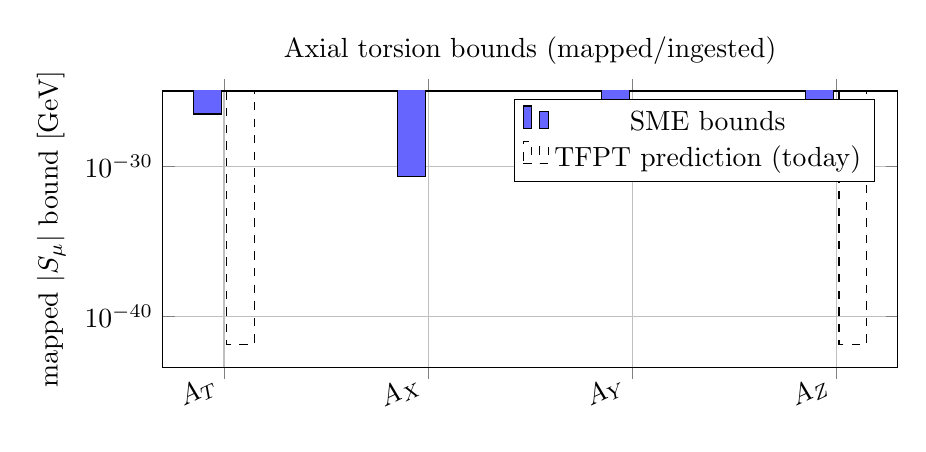
\begin{tikzpicture}
\begin{axis}[
    ybar,
    ymode=log,
    width=0.9\linewidth,
    height=0.42\linewidth,
    ylabel={mapped $|S_\mu|$ bound [GeV]},
    title={Axial torsion bounds (mapped/ingested)},
    symbolic x coords={AT,AX,AY,AZ},
    xtick=data,
    xticklabel style={rotate=25,anchor=east},
    xticklabels={$A_T$,$A_X$,$A_Y$,$A_Z$},
    grid=major,
    legend pos=north east
]
\addplot[fill=blue!60] coordinates {(AT,2.9e-27) (AX,2.1e-31) (AY,2.5e-31) (AZ,1.0e-29)};
\addlegendentry{SME bounds}
\addplot[black, dashed] coordinates {(AT,1.436869415091482e-42) (AZ,1.436869415091482e-42)};
\addlegendentry{TFPT prediction (today)}
\end{axis}
\end{tikzpicture}
\caption{Axial torsion bounds (mapped). SME coefficients $A_\mu$ (x-axis labels) translated to $|S_\mu|$ with explicit mapping; the TFPT baseline $S_\mu(\text{today})=0$ is shown at a small floor value for the log scale.}
\label{fig:torsion-bounds}
\end{figure}

\begin{tcolorbox}[colback=gray!5, colframe=gray!60,
    title={\textbf{Two concrete torsion test benchmarks (suite; regime designer)}}, fonttitle=\bfseries\small]
The suite includes an explicit ``regime designer'' that translates spin-polarized media into a toy torsion estimate and compares it to vetted component-wise bounds (module \texttt{ux\_torsion\_regime\_designer}). 
The intent is not to claim a derived microscopic coupling here, but to make \emph{testability regimes} concrete.
\end{tcolorbox}

\begin{table}[H]
\centering
\begin{tabular}{@{}llll@{}}
\toprule
\textbf{Benchmark} & \textbf{Coupling scale} & \textbf{Density} & \textbf{$|S_\mu|$ for $c_{\rm spin}=1$ [GeV]} \\
\midrule
Electron gas (lab) & $M_{\rm Pl}^{-1}$ & $n\sim 10^{23}\,\mathrm{cm^{-3}}$ & $\sim \num{3.24e-56}$ \\
Nuclear matter core & TFPT $M^{-1}$ & $n\sim 0.16\,\mathrm{fm^{-3}}$ & $\sim \num{3.28e-31}$ \\
\bottomrule
\end{tabular}
\caption{Order-of-magnitude torsion benchmarks from the suite module \texttt{ux\_torsion\_regime\_designer}. In the lab benchmark, the signal is hopelessly small under Planck coupling; in dense matter under TFPT-$M$ coupling, the estimate approaches current bounds (depending on the effective $c_{\rm spin}$).}
\end{table}

\begin{figure}[H]
\centering
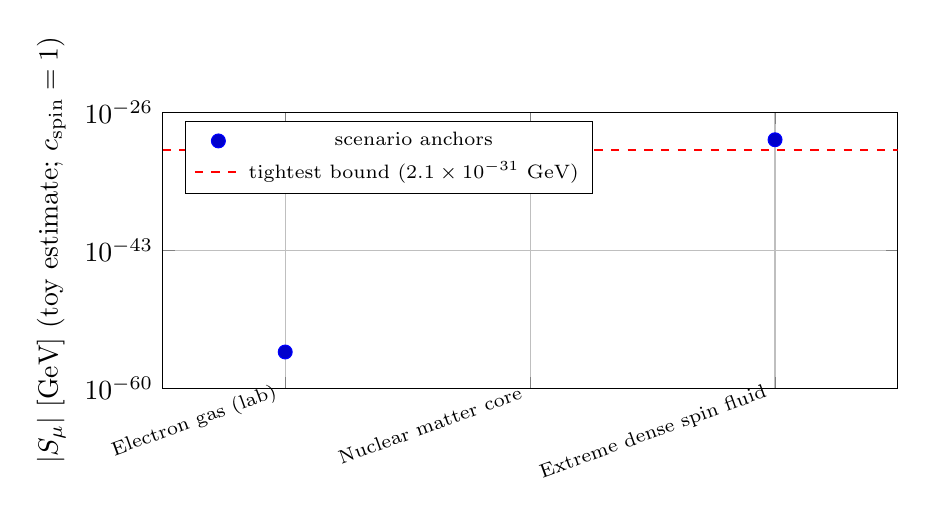
\begin{tikzpicture}
\begin{axis}[
    width=0.9\linewidth,
    height=0.42\linewidth,
    ymode=log,
    ymin=1e-60, ymax=1e-26,
    xmin=0.5, xmax=3.5,
    xtick={1,2,3},
    xticklabels={Electron gas (lab), Nuclear matter core, Extreme dense spin fluid},
    x tick label style={rotate=20, anchor=east, font=\scriptsize},
    ylabel={$|S_\mu|$ [GeV] (toy estimate; $c_{\rm spin}=1$)},
    grid=both,
    legend style={font=\scriptsize},
    legend pos=north west,
]
\addplot+[only marks, mark=*, mark size=2.5pt] coordinates {
    (1,3.2396753580225e-56)
    (2,3.2832238430084956e-31)
    (3,4.104029803760619e-30)
};
\addlegendentry{scenario anchors}

\addplot[red, dashed, thick] coordinates {(0.5,2.1e-31) (3.5,2.1e-31)};
\addlegendentry{tightest bound ($2.1\times10^{-31}$ GeV)}
\end{axis}
\end{tikzpicture}
\caption{Suite regime scan (\texttt{ux\_torsion\_regime\_designer}): torsion estimates and bound-saturation targets across illustrative spin-medium scenarios.}
\end{figure}

%-----------------------------------------------------------------------------
\subsubsection{Achromatic polarization rotation around compact objects (EHT intercept test)}
\label{sec:eht-intercept}
%-----------------------------------------------------------------------------

Beyond the cosmic birefringence prediction (Theorem~\ref{thm:birefringence}), TFPT implies a local, achromatic polarization rotation
in the presence of a nonzero $E\cdot B$ environment (see the companion note \cite{bhAchromaticRotationNote2025}). EHT-style polarimetry
provides the relevant data products for such an intercept test \cite{ehtm87pol2021}. A simple dyonic toy model yields
\begin{equation}
\beta_{\mathrm{BH}}(r_{\mathrm{em}})
:= \frac{1}{256\pi^4}\,\frac{Q^{\mathrm{eff}}_e Q^{\mathrm{eff}}_m}{r_{\mathrm{em}}^2},
\end{equation}
where $r_{\mathrm{em}}$ is the emission radius and $Q^{\mathrm{eff}}_{e,m}$ denote effective electromagnetic charges sourcing $E\cdot B$ along the line of sight. A toy derivation of the $1/r^2$ scaling is given in Appendix~\ref{app:bh-dyonic}.

\textbf{Observation strategy (EHT style).}
At each image pixel $x$, fit the electric vector position angle (EVPA) across frequencies by
\begin{equation}
\chi(\lambda^2,x)=\chi_0(x)+\mathrm{RM}(x)\lambda^2,
\end{equation}
and interpret $\chi_0(x)$ as the achromatic intercept map. A nonzero intercept pattern correlated
with emission radius and polarization structure provides a direct falsifiable test.

\begin{tcolorbox}[colback=gray!5, colframe=gray!60, breakable,
title={\textbf{EHT Intercept Map Procedure (achromatic intercept $\chi_0$)}}, fonttitle=\bfseries\small]
\begin{itemize}[leftmargin=1.5em, topsep=2pt, itemsep=2pt]
    \item For each pixel $x$, fit $\chi(\lambda^2,x)$ across bands to $\chi_0(x)+\mathrm{RM}(x)\lambda^2$.
    \item Treat $\chi_0(x)$ as the \emph{achromatic} intercept map (TFPT observable).
    \item Treat $\mathrm{RM}(x)$ as a Faraday-rotation nuisance map (astrophysical foreground / plasma).
    \item The primary null test is $\chi_0(x)=0$ (up to instrumental calibration); a robust nonzero pattern is the signal channel.
    \item Achromaticity check: $\chi_0(x)$ is stable under band splits; residual frequency dependence belongs in $\mathrm{RM}(x)$.
    \item Control sources: apply the same fit to calibrators or off-source regions; expect $\chi_0(x)\approx 0$.
    \item Sign/handedness check: a parity flip or Stokes $Q/U$ sign inversion should flip $\chi_0$; failure indicates systematics.
\end{itemize}
\end{tcolorbox}

\begin{figure}[H]
\centering
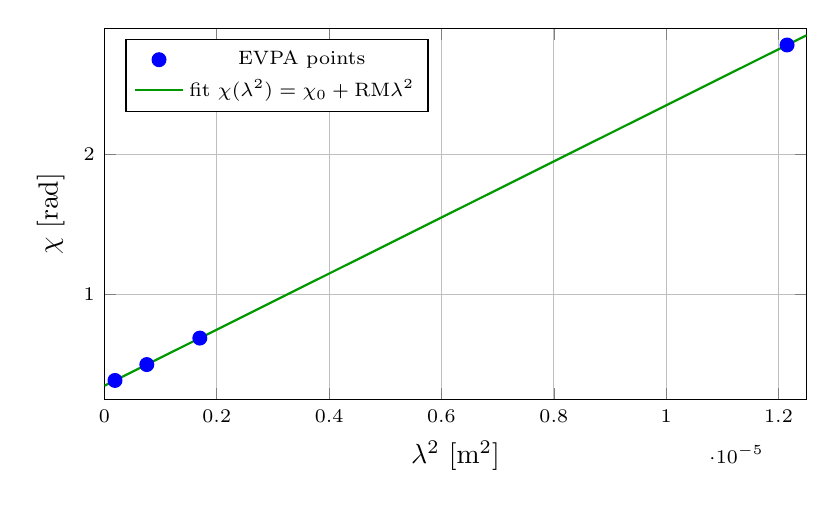
\begin{tikzpicture}
\begin{axis}[
    width=10.5cm, height=6.3cm,
    xlabel={$\lambda^2$ [m$^2$]},
    ylabel={$\chi$ [rad]},
    xmin=0, xmax=1.25e-5,
    ymin=0.25, ymax=2.9,
    grid=major,
    scaled x ticks=true,
    tick label style={font=\scriptsize},
    legend style={font=\scriptsize},
    legend pos=north west
]
    \addplot[only marks, mark=*, mark size=2.5pt, blue] coordinates {
        (1.215190885258e-05,2.780382)
        (1.698970092130e-06,0.689794)
        (7.550978187245e-07,0.501020)
        (1.887744546811e-07,0.387755)
    };
    \addlegendentry{EVPA points}

    \addplot[thick, green!60!black] coordinates {(0,0.35) (1.25e-5,2.85)};
    \addlegendentry{fit $\chi(\lambda^2)=\chi_0+\mathrm{RM}\lambda^2$}

    \node[anchor=south west, font=\scriptsize] at (axis cs:0.25e-6,2.55) {$\chi_0\neq 0$};
\end{axis}
\end{tikzpicture}
\caption{Schematic EVPA fit: an achromatic intercept $\chi_0$ plus a Faraday term $\mathrm{RM}\lambda^2$. The intercept map extracted from multi-frequency imaging is the primary TFPT observable.}
\label{fig:evpa_intercept}
\end{figure}

\paragraph{Sensitivity requirements.}
A Monte Carlo forecast quantifies the noise and calibration requirements for
EHT detection of the TFPT intercept signal $\chi_0\approx 4.2$~mrad:

\begin{figure}[H]
\centering
\begin{tikzpicture}
\begin{groupplot}[
    group style={group size=2 by 1, horizontal sep=1.5cm},
    width=0.44\linewidth, height=0.36\linewidth
]
\nextgroupplot[
    xlabel={noise $\sigma$ (rad)},
    ylabel={SNR},
    title={Detection SNR vs noise},
    xmode=log, ymode=log,
    grid=major,
    legend pos=north east
]
\addplot+[mark=o, thick] coordinates {
    (0.001,6.568) (0.005,1.344) (0.01,0.693)
    (0.02,0.322) (0.05,0.133) (0.1,0.071) (0.2,0.033)
};
\addlegendentry{SNR}
\addplot[red, dashed] coordinates {(0.001,3) (0.2,3)};
\addlegendentry{$3\sigma$ threshold}

\nextgroupplot[
    xlabel={calibration offset (rad)},
    ylabel={bias / signal},
    title={Calibration bias},
    grid=major,
]
\addplot+[mark=square, thick] coordinates {
    (0.0,0.023) (0.001,0.223) (0.005,1.251)
    (0.01,2.453) (0.02,4.954)
};
\addplot[red, dashed] coordinates {(0,1) (0.02,1)};
\addlegendentry{bias $=$ signal}
\end{groupplot}
\end{tikzpicture}
\caption{EHT intercept detectability.
  Left: $3\sigma$ detection requires $\sigma_{\text{noise}} < 1$~mrad.
  Right: calibration offset must stay below $\sim5$~mrad to avoid
  bias exceeding the signal.}
\label{fig:eht-sensitivity}
\end{figure}

%-----------------------------------------------------------------------------
